\documentclass[11pt]{article}
\usepackage[margin=1in]{geometry}
\usepackage{amsmath}
\usepackage{booktabs}
\usepackage{hyperref}
\usepackage{graphicx}
\graphicspath{{images/}{../frontend/public/}}
\usepackage{soul}
\usepackage{tabularx}
\usepackage{xcolor}
\sethlcolor{yellow} % default is yellow

\input{githash}

\title{A Bayesian inference method for estimation of soil water content with low-cost capacitive moisture sensor data}
\author{%

\includegraphics[height=1.5cm]{images/teal-no-bg-dark-256.png}\\[6pt]
Alex Southgate\\
Biosystemau De Cymru | South Wales Biosystems \\
\texttt{alex.southgate@biosystemau.cymru}
}
\author{
  Alex J. Southgate$^{1,*}$ \\[1em]
  \small $^{1}$Cardiff University, Cardiff, United Kingdom \\
  \small $^{*}$Corresponding author: southgateJA@cardiff.ac.uk
}
\date{\today}


\date{\today}

\begin{document}
\maketitle

\begin{abstract}

Climate change represents a challenge to food security by interfering with the environmental conditions needed for productive plant growth. While technology can be used for partial mitigation, access to technology is inequitable. Low-cost microntrollers, such as the ESP32, have recently lowered the barrier for entry into prototyping smart devices. ESP32s equipped with capacitive moisture sensors have been suggested for low-cost smart plant watering systems. However, measuring moisture in soil is complex, potentially destructive, and requires careful calibration in order to characterise the response curve mapping soil water content to sensor measurements. Here, we developed a Bayesian method for estimating the inverse response curve from capacitive moisture sensor data, known water doses, and prior uncertainty, bypassing the need for destructive gravimetry. This method constitutes the core calibration module of the open-source \textit{OpenHCult} software system for low-cost horticultural automation.

\end{abstract}

\section{Introduction}

Recent work has proposed the use of ESP32-class microcontrollers and low-cost moisture sensors for automated watering systems and measurement of soil water content (SWC) \cite{biswas2018-solar-pump, purnomo2021-lora, sudarmaji2024-smart-soil, afzal2025-arima}, motivated by mitigating water shortages \cite{afzal2025-arima}, with increased interest in application of IoT sensors to agriculture \cite{ruiz2025-iot-mapping}. As global warming continues, both flooding and water shortages are increasing world-wide \cite{ficklin2022hydrological}, including in the United Kingdom \cite{lane2021climate}. In previous work, ESP32/capacitive sensor calibration and validation has been performed by gravimetry \cite{sudarmaji2024-smart-soil}. However, it is expected that calibrated response curves depend on a range of factors, including soil type (i.e. clay content), and temperature \cite{merlin2007-calibration}. Furthermore, end users may find it difficult to undertake calibration for each specific application type. 

Typically, gravimetric sampling can be used to characterise SWC, but is destructive and time consuming; this process often involves drying soil by heating and therefore cannot be easily applied to existing plant systems. Capacitive moisture sensors, as with all electromagnetic methods (EM) measure SWC indirectly through the dielectric permittivity \cite{kelleners2005-frequency-dependence}, though it is dependent on measurement electrical frequency \cite{kelleners2005-frequency-dependence,sheng2025-frequency} and temperature \cite{jones2005-em-methodology}. Field capacity (FC), the water content at which internal drainage stops, is often utilized \cite{jury2004soil}. 

Ideal ranges for SWC varies across plant species and growth stages. For example, tomatoes (\textit{Lycopersicon esculentum}) may grow best at 70\% field capacity (FC) \cite{liu2019tomato}, while the cactus \textit{Opuntia ficus-indica} was shown to exhibit stress under 30\% FC \cite{lahbouki2023effects}.

Existing work has been undertaken on moisture sensor calibration and characterisation of variability. Bogena et al (2017) \cite{bogena2017-calibration} developed a procedure for calibration of low-cost SMT1000 moisture sensors and undertook systematic calibration of hundreds of sensors in a range of media, observing sensor-to-sensor variability and both density and temperature dependence. In contrast, Kizito et al. (2008) \cite{kizito2008-frequency} found that for research-grade ECH2O probes (Decagon Devices Inc., Pullman, WA) with a measurement frequency of 70 MHz, a single calibration curve was sufficient for relating electrical conductivity to SWC across different soil salinities, though they did find variability with the degree of probe immersion and dependency of measurements on temperature, and the sensors used are more an order of magnitude more costly than the capacitive sensors used in other studies (e.g. \cite{sudarmaji2024-smart-soil}). While cheap, these capacitive sensors can be reliable given controls on soil type and the ratio of solid matter to volume \cite{placidi2020characterization}.

The objective of this work was to introduce an automated system and statistical method for automated calibration of sensors using watering volume data (dosage) rather than labour intensive gravimetric calibration. This aim was primarily motivated by the challenge end users may find with gravimetric calibration, as well as lack of generalisability of a given calibration curve.

\section{Methods}

\subsection{Pre-processing}

Irregularly spaced sensor data gathered from sensors was smoothed with an exponential moving average \cite{genccay2001introduction} (or exponentially weighted moving average (EWMA) \cite{zumbach2001operators}), a single-pole low-pass filter \cite{smith1997scientist} with time-weighted coefficients:

\[
\tilde{X}_{t_i} = e^{-\Delta t/\tau} \tilde{X}_{t_{i-1}} + (1-e^{-\Delta t/\tau}) X_{t_i}
\]

Smoothed data was used primarily for velocity calculations, as described below.

\subsection{Calibration}

\subsubsection{Integral data and the inverse response function}

For sensor index $i$ and time $t$, let $T_t$ be the total water volume, $Y_{i,t}$ the relative (here volumetric) SWC local to sensor $i$, and $X_{i, t} = h(Y_{i,t})$ the sensor response. Let $V$ be the container volume, and therefore $T_t/V$ the average volumetric SWC. $Y_t$ and $T_t$ cannot be measured directly non-destructively. If the inverse response function $h^{-1}$ is known, $Y_{i,t} = h^{-1}(X_{i,t})$ could be computed. For multiple sensors, $T_t$ and average volumetric SWC can be computed by averaging over $N$ sensors, assuming sensors are uniformly distributed in the soil:

\begin{equation}
T_t = \int_{\Omega} Y(\omega) d\omega \approx \frac{V}{N} \sum_{i=1}^N Y_{i,t}
\end{equation}

Since the response function can depend on both soil parameters, environmental factors, and sensor parameters including placement (e.g. how densely packed soil is around the sensor), we assume it is unknown and aim to estimate it. \\

$\Delta T$, the change in total system water, is measurable for watering events that are recorded, which provides information on the response function. For example, if the inverse response was linear, assuming no noise, the slope $T = Vh^{-1}(X)$ could be reconstructed from $(X_{i, start}, X_{i, end}, \Delta T)$, and the intercept from a single measurement $X_i = h^{-1}(0)$. In practice, the response curve is non-linear, and plants are usually sensitive to water content, tolerating only a narrow range of saturation, so the values $(X_{i,start}, X_{i,end}, \Delta Y_i)$ are drawn from a narrow range of the domain. As such, only a narrow section of the curve $h^{-1}$ can be sampled. \\

\subsubsection{Combining sensor estimates}

Each sensor has its own local saturation $g_j(x)$, determined by physical heterogeneity. At the same time, the total water content of the container is a global property of the system. Our method estimates, per sensor, the total water content. Given $N$ sensors with voltage measurement vector $\mathbf{x}$. Each inverse sensor response is itself a random variable. We refine our single-sensor model as:

\begin{equation}
SWC(\mathbf{x}) = S \cdot E[g(\mathbf{x})] \approx \frac{S}{N}\sum_{j=1}^N g_j(x_j)
\end{equation}

allowing $S$, a global quantity to be estimated jointly, with separate estimates for the local relative saturation functions $g$ per-sensor.

\subsubsection{Model}

In order to resolve these issues, a parametric form for $h^{-1}$ can be assumed. The sensor response has two plateaus, one at dry (low SWC) and one at wet (high SWC). Different functions may perform better for different subsets of the domain. To model this, we consider two components: an exponential shape with a maximum of $1$, which may differ between sensors, and be informed by both a prior normalized calibration curve and $\Delta T$, and a joint scale, which is informed by $\Delta T$. We use an exponential shape and do not attempt to model the dry end shape, instead using an intercept term. Given that the response function becomes flat at saturation, the inverse response function becomes vertical at full saturation. We do not attempt to extrapolate beyond the measured sensor minimum because small errors in assumed $X_{min}$, which may vary between sensors, can result in large errors in estimated SWC where the curve is nearly vertical. 

\begin{equation}
h^{-1}(X_t) = S \cdot g(X_t) = S \cdot \Big((1-q_{dry})\exp\Big\{-k (1 - u(X_t; x_{wet}, x_{dry})\Big\} + q_{dry}\Big)
\end{equation}

Where $u(X_t)$ is a rescaling of $[x_{wet}, x_{dry}]$ to the interval $[0, 1]$. The shape intercept parameter $q_{dry}$ allows the normalized curve $g(x)$ to be squashed into the interval $[q_{dry}, 1.0]$. The parameter $S$ is equal to the total water volume at the minimum sensor measurement, and can be related to volumetric SWC as:\\

\begin{equation}
SWC_{xmin} = S / V
\end{equation}

\subsubsection{Bayesian estimation}

To combine the chord data $(X_{i, start}, X_{i, end}, \Delta T)$, dry anchor sample $X_i(0) = h^{-1}(T=0)$, prior assumptions on the parametric form of $h^{-1}$, optional prior calibration points, and the unknown scale parameter $S$, we adopt a Bayesian framework. We assume lognormal dosage samples:

\begin{equation}
\log(\Delta T) \sim Normal(\log (h^{-1}(X_{i, end}; S, k) - h^{-1}(X_{i, start}; S, k)), \sigma^2)
\end{equation}

With the target parameters $\theta = (S, k, \sigma^2)$. Priors on the lower bound $x_{wet}$ are taken as uniform on a user-specified interval.

\begin{table}[ht]
    \centering
    \small % Slightly smaller font to help with density
    \caption{Summary of Prior Distributions for Model Parameters}
    \label{tab:priors}
    % Specify the width as \textwidth
    \begin{tabularx}{\textwidth}{llX} 
        \toprule
        \textbf{Parameter} & \textbf{Prior Distribution} & \textbf{Description} \\
        \midrule
        $S$ (Scale) & Normal & Weakly informative; roughly estimated by user \\
        $k$ (Exp. shape) & Improper & Unconstrained shape, unintuitive for user \\
        $q_{dry}$ (Intercept) & Uniform(0, 0.5) & User-specified, default chosen from experiment \\
        $\sigma^2$ (Variance) & Improper & Accommodates noise sources including error in water measurement \\
        \bottomrule
    \end{tabularx}
\end{table}

Estimation is performed with the \textit{emcee} \cite{foreman2013emcee} package in Python. Given posterior samples, volumetric SWC is estimated by Monte Carlo sampling, given the independence of $V$ and calibration model parameters. For each SWC sample, velocity is computed, from which credible intervals can be calculated. In order to accommodate step changes in velocity under watering and drying conditions, as well as small velocities during drying, velocity is assumed to be piecewise-constant, and computed from $\ell_1$ trend filtered \cite{kim2009ell_1} posterior SWC samples, since penalising the acceleration enforces piecewise constant velocity. \textit{cvxpy} \cite{diamond2016cvxpy} was used with objective:

\begin{equation}
\min_z \Big(||z-SWC||^2_2 + \lambda ||D_2 z||_1\Big)
\end{equation}

In principle this objective is opposed to EWMA smoothing, and since only two regimes are of interest (fast watering and slow drying), this is used as a convenience.

\section{Results}

\begin{figure}[!ht]
  \centering
  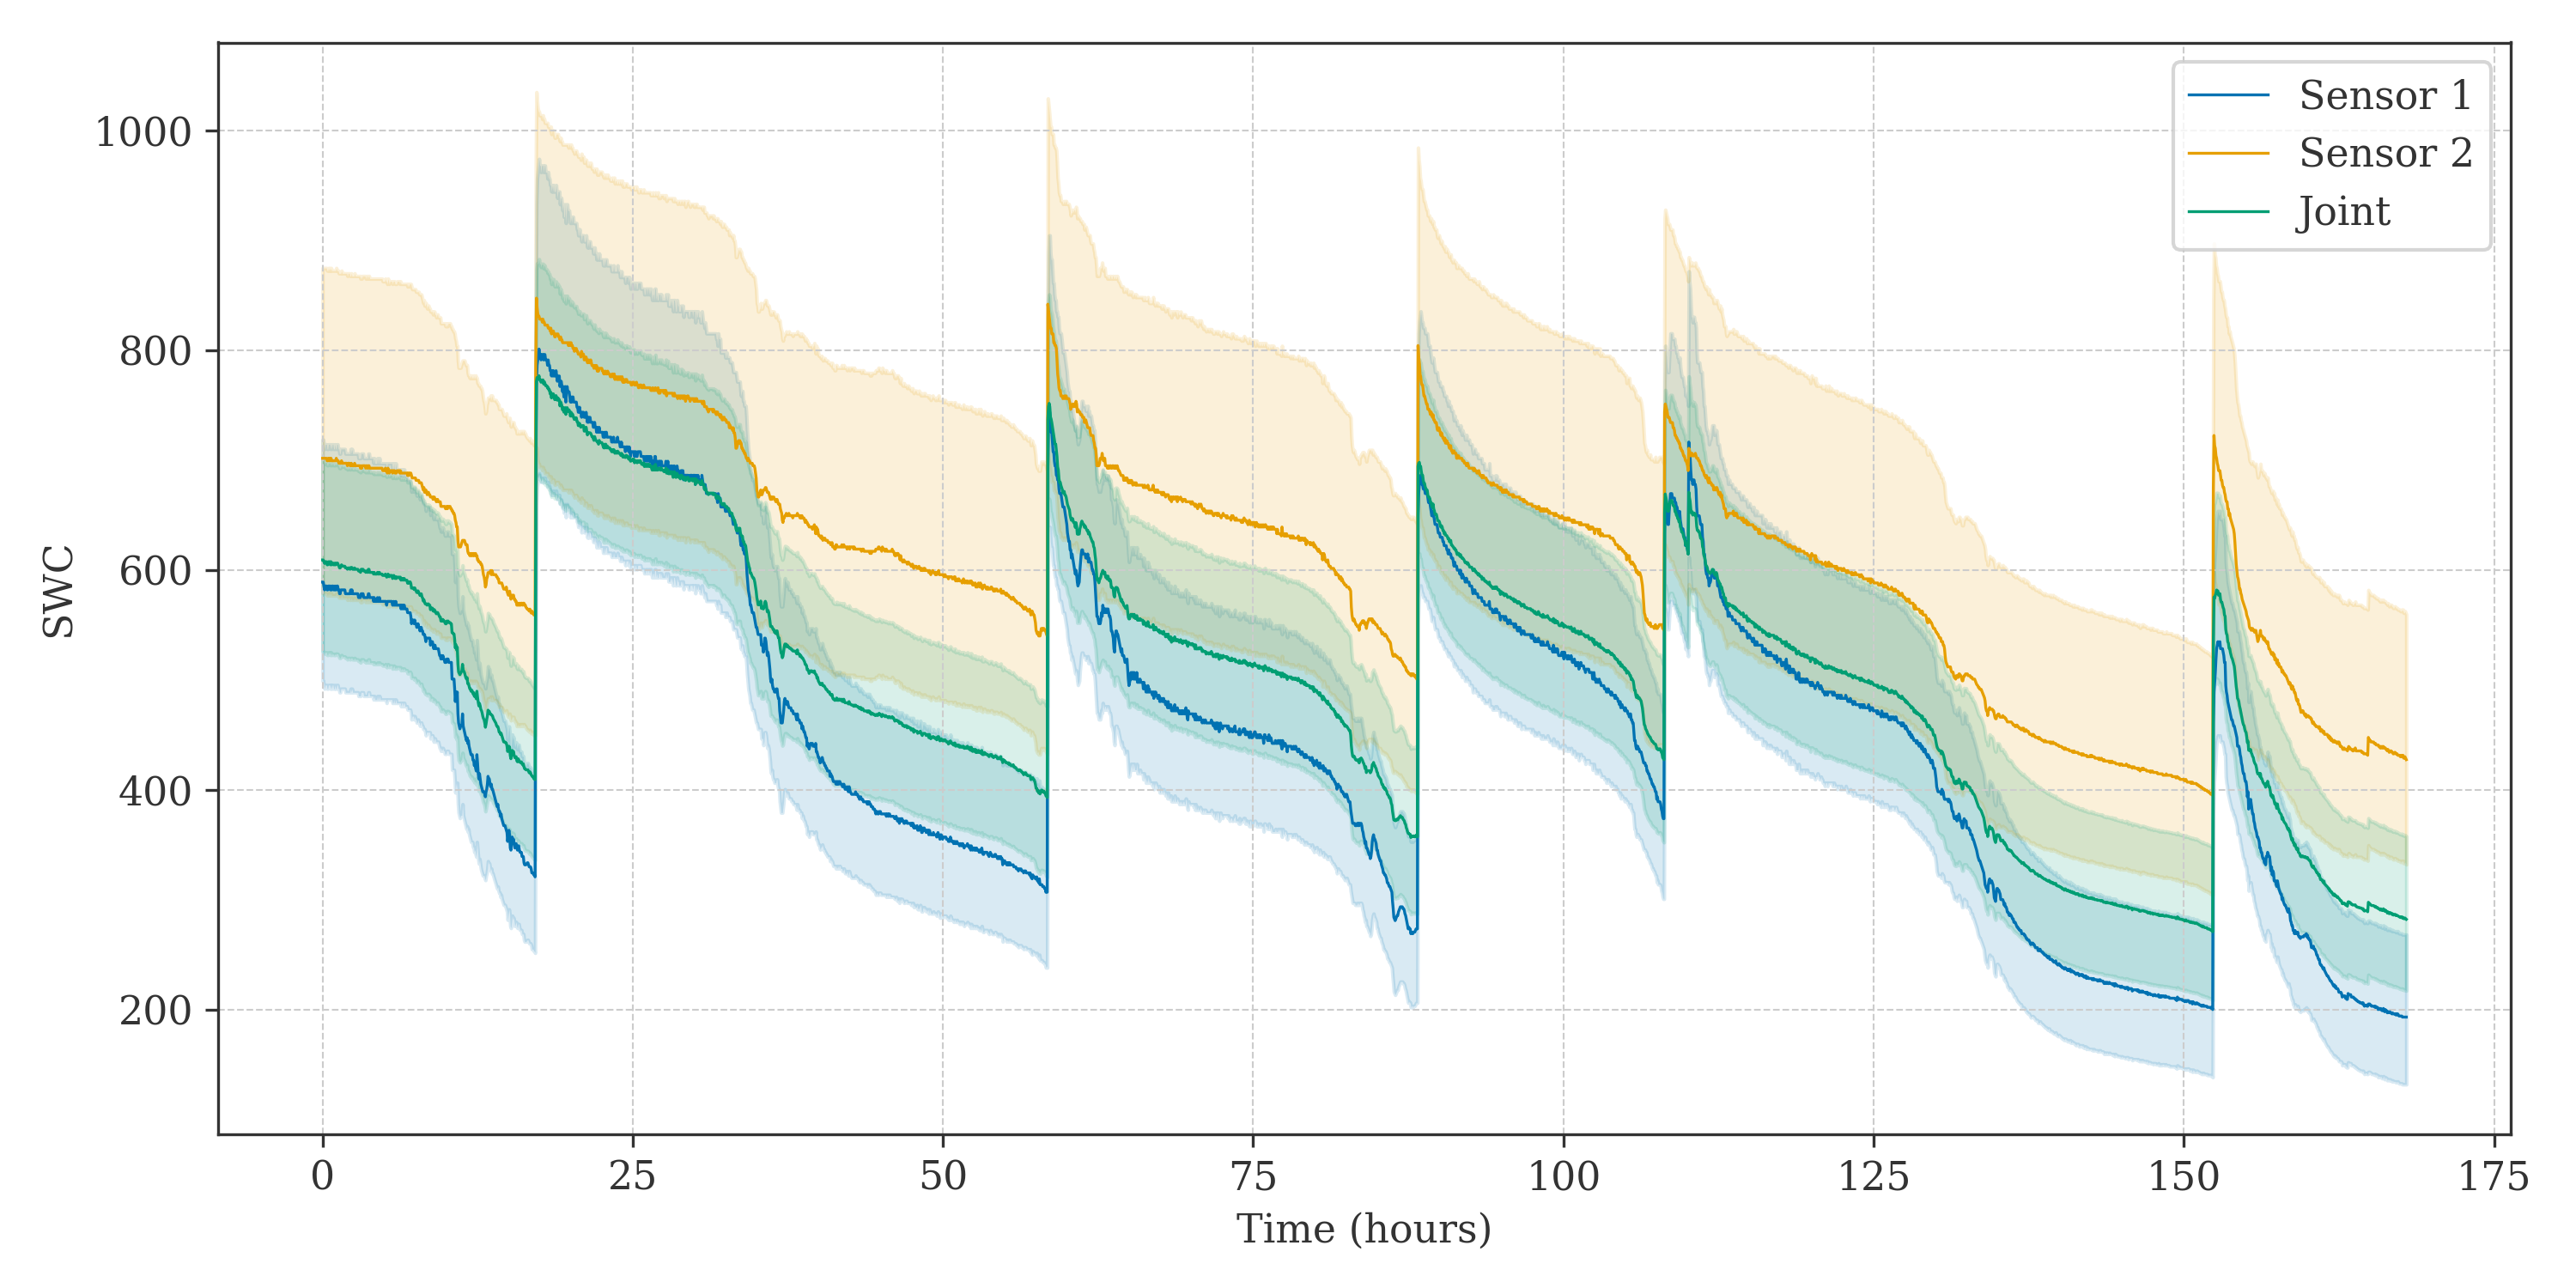
\includegraphics[width=1.0\linewidth]{images/real_data_timeseries.png}
  \caption{Estimated SWC over time from multi-sensor Bayesian calibration. Individual sensor posteriors (thin lines with shaded 95\% CI) and joint posterior (bold line with shaded CI).}
  \label{fig:timeseries}
  \end{figure}

\begin{figure}[!ht]
  \centering
  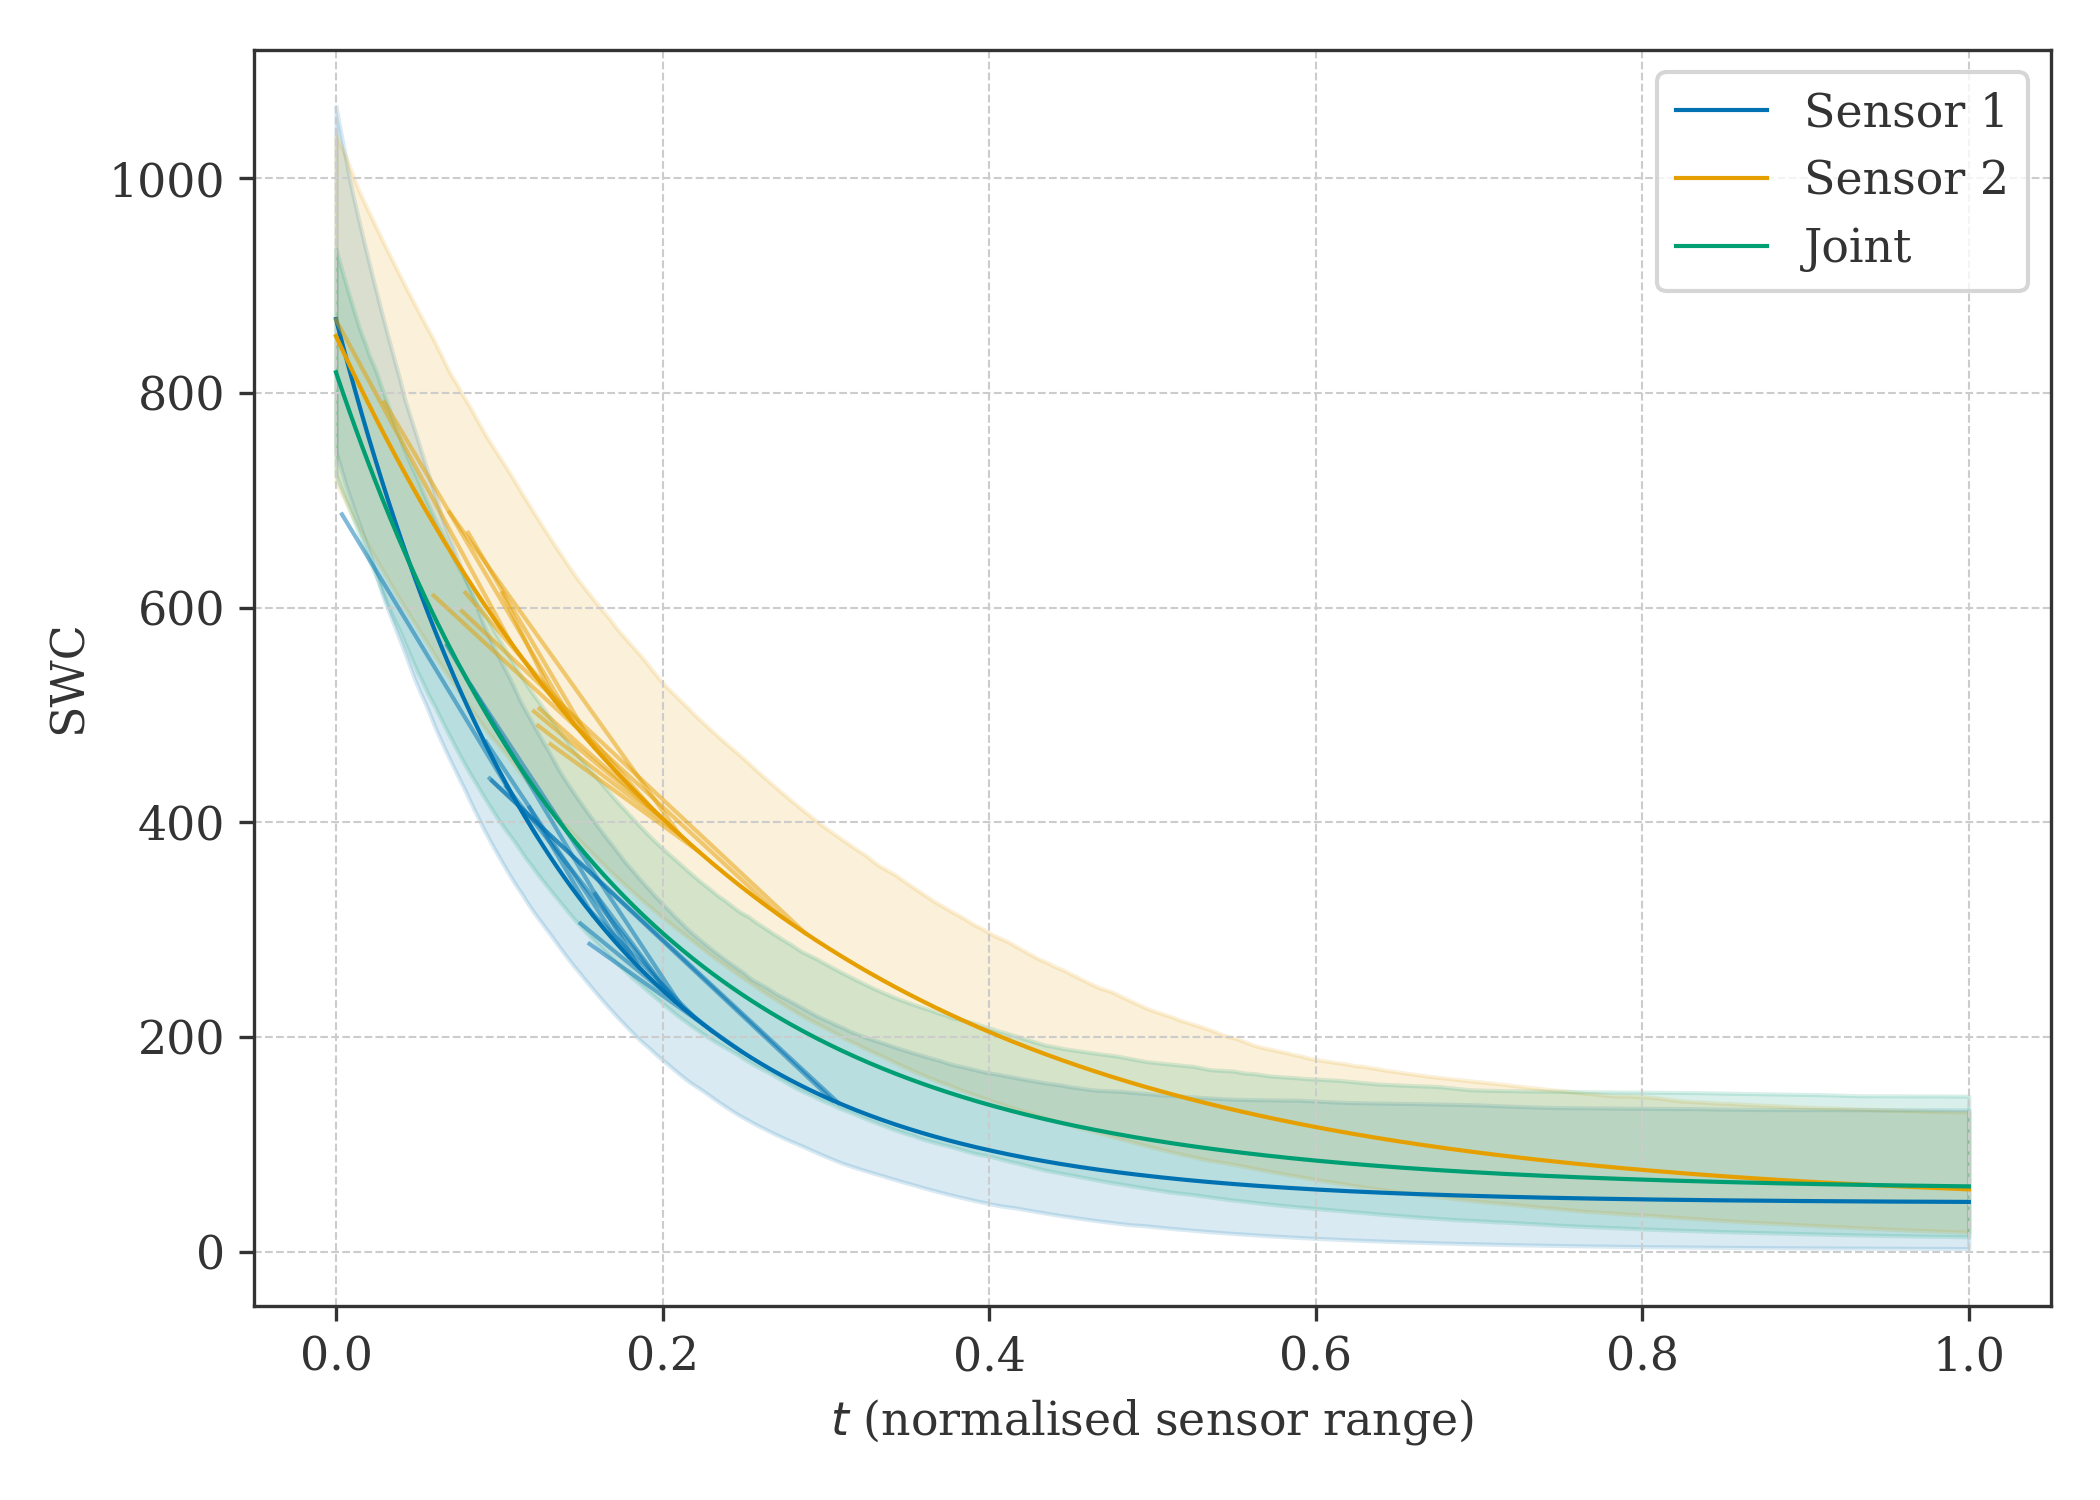
\includegraphics[width=0.85\linewidth]{images/real_data_calibration.png}
  \caption{Calibration (response) curves per sensor and joint calibration, plotted parametrically against normalised sensor range $t \in [0,1]$. Chord segments show the observed watering events. Shading shows 95\% credible intervals.}
  \label{fig:calibration}
\end{figure}

\begin{figure}[!ht]
  \centering
  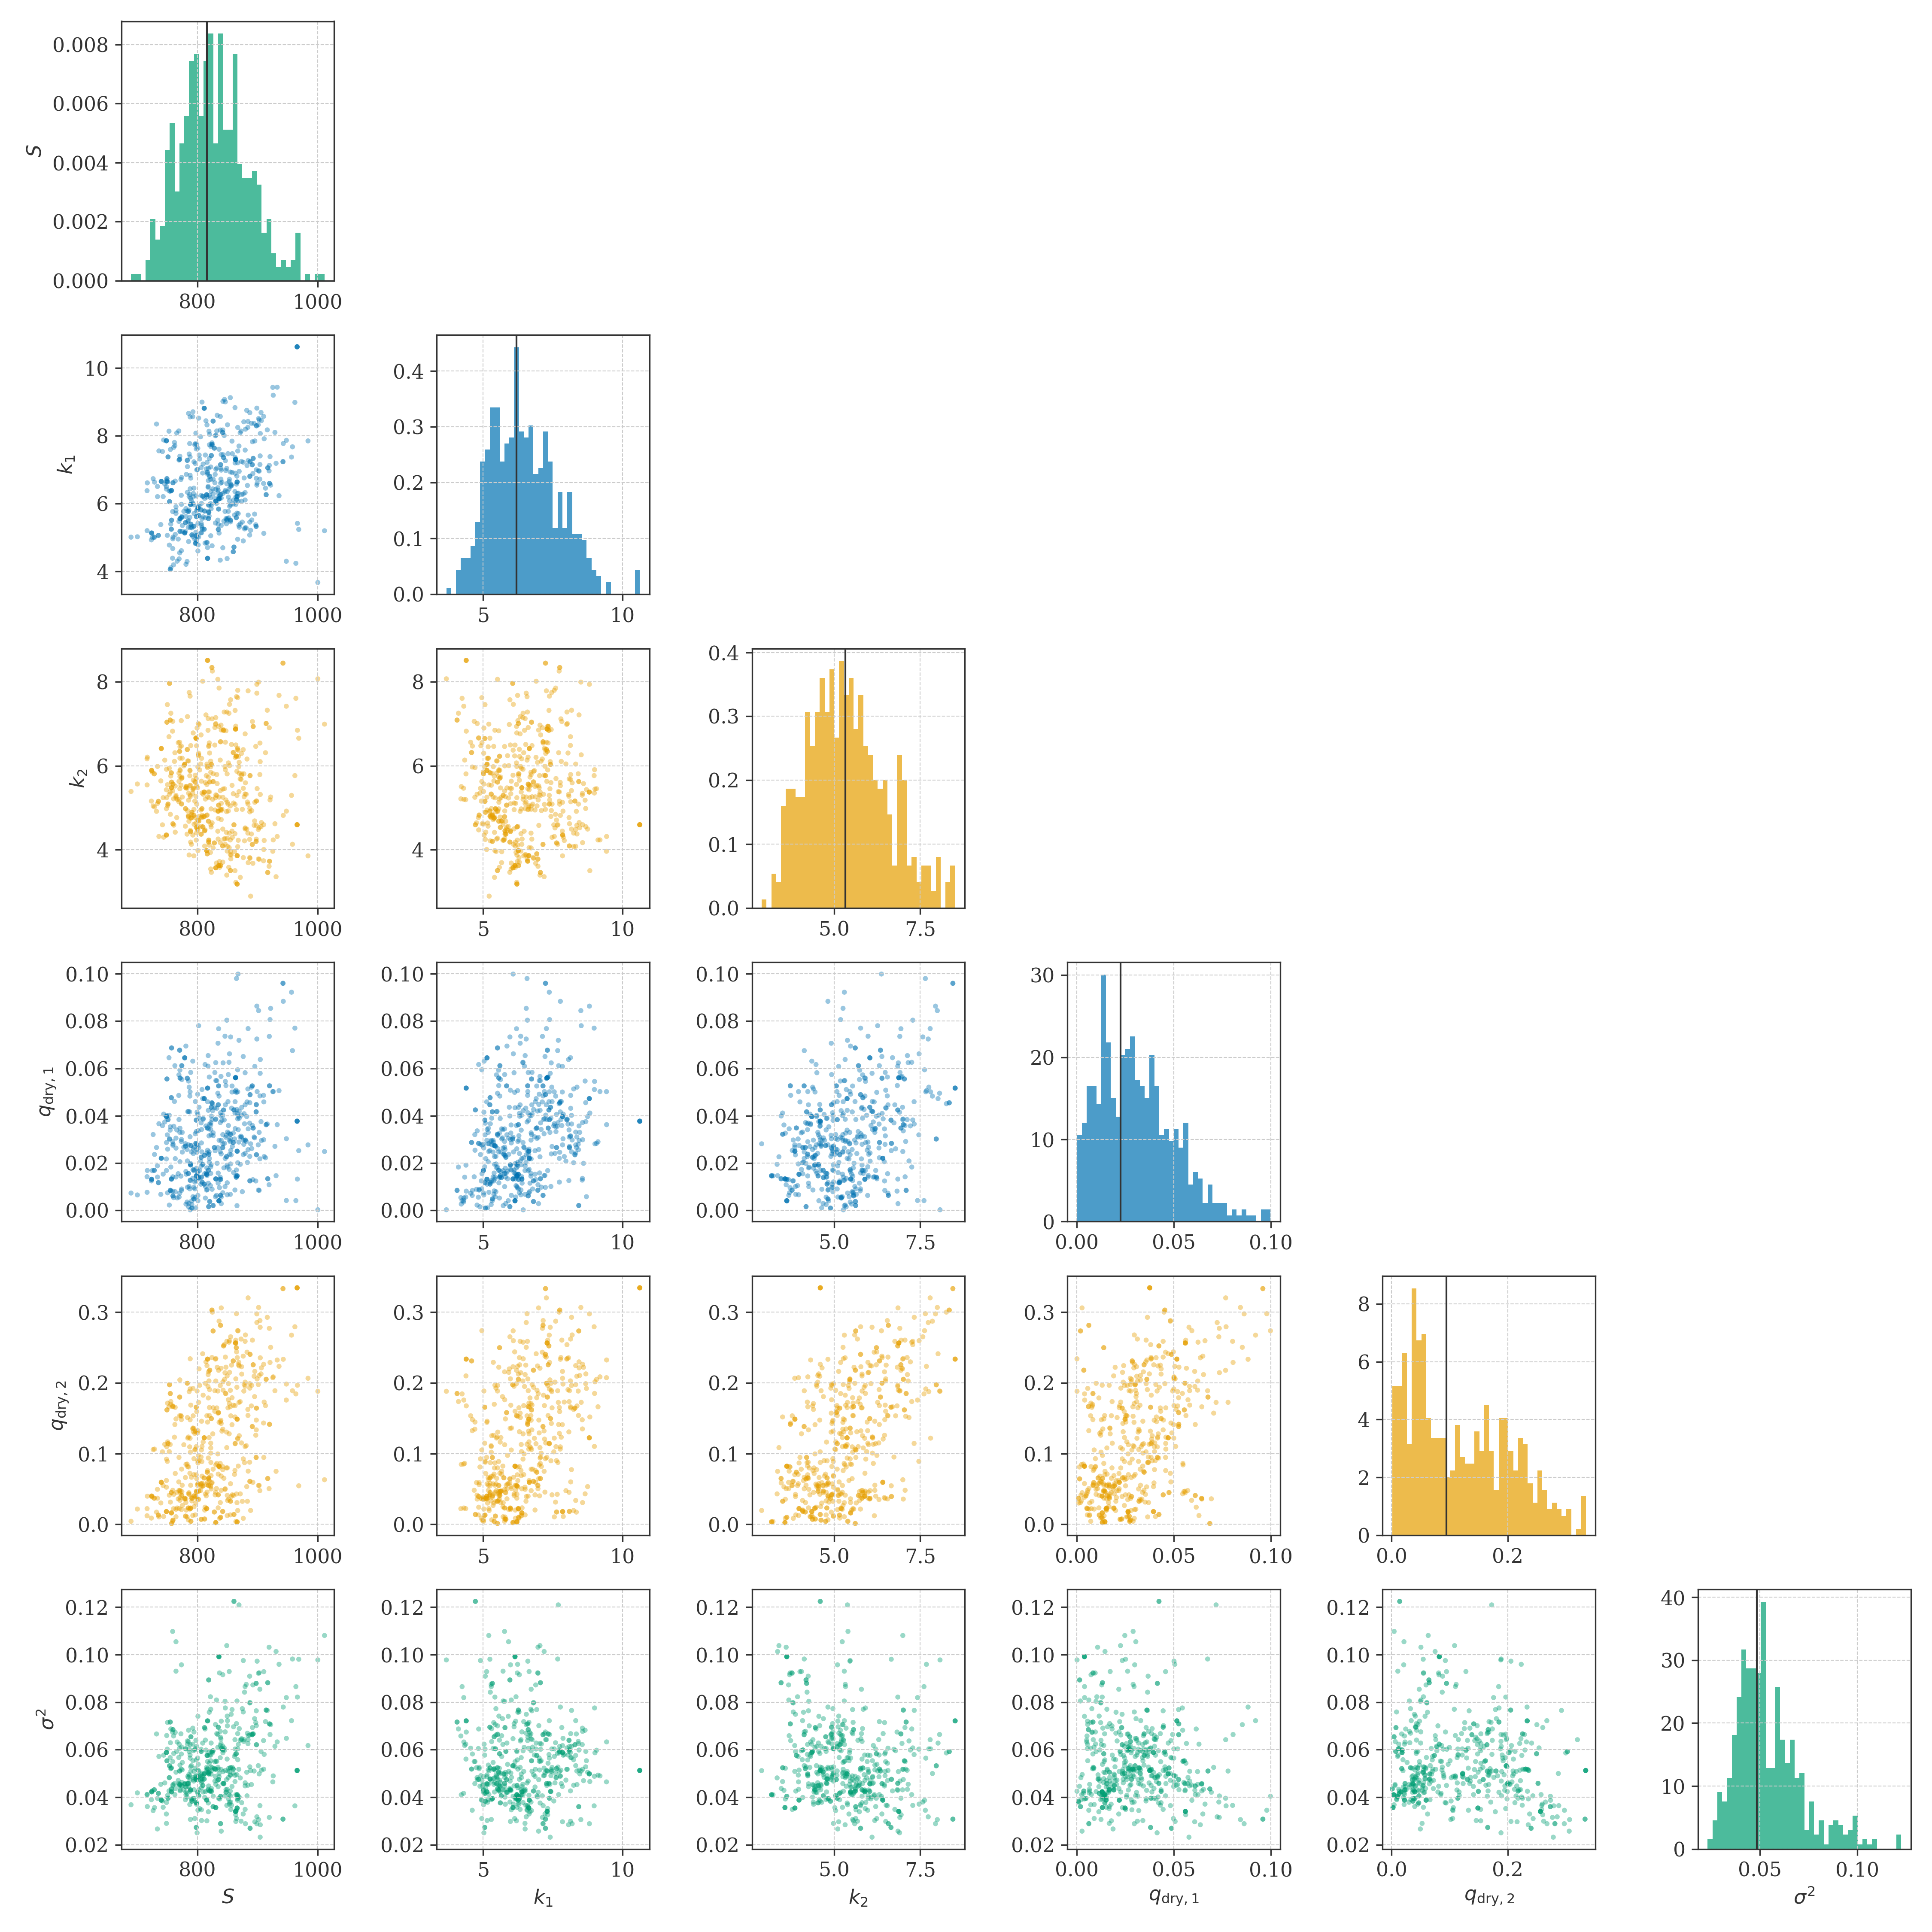
\includegraphics[width=0.9\linewidth]{images/real_data_corner.png}
  \caption{Posterior parameter correlations from joint MCMC calibration. Diagonal panels show marginal distributions; lower triangle shows pairwise scatter plots.}
  \label{fig:corner}
\end{figure}

\section{Discussion}

Capacitive moisture sensors are sensitive to positioning in the soil. In order to account for blips and noise in the sensor data, such as from mechanical touch, EWMA smoothing is used.
Without smoothing, posterior SWC samples are noisy, and during drying, values are both small and fluctuate above and below zero. Although smoothing allows consistent values, such as 
a small but negative derivative in SWC, in principle this objective is opposed to the $\ell_1$ trend filtering used for discretisation of the velocity since step changes are smoothed out.
In practice, the $\ell_1$ segmentation is just used to accommodate both high, positive rates during watering and small negative rates during drying. In future, other modelling approaches could be used
without this contrasting objective. 

\section{Appendix}

\bibliographystyle{plain}
\bibliography{references}

\end{document}
